\tikzset{every picture/.style={line width=0.75pt}} %set default line width to 0.75pt        

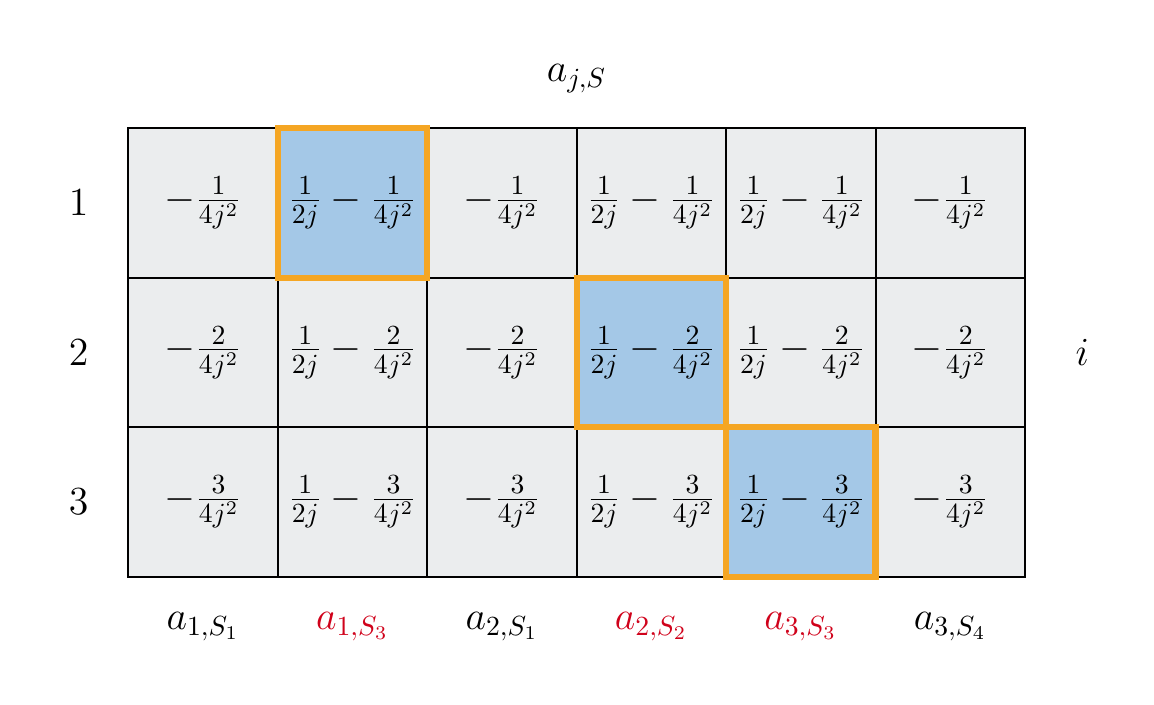
\begin{tikzpicture}[x=0.75pt,y=0.75pt,yscale=-1.2,xscale=1.2]
%uncomment if require: \path (0,447); %set diagram left start at 0, and has height of 447

\definecolor{niceRed}{RGB}{190,38,38}
\definecolor{Red2}{RGB}{219, 50, 54}
\definecolor{mgreen}{RGB}{160, 200, 140}
\definecolor{blueGrotto}{RGB}{5,157,192}
\definecolor{limeGreen}{HTML}{81B622}
\definecolor{myellow}{rgb}{0.88,0.61,0.14}
\definecolor{darkGreen}{HTML}{2E8B57}
\definecolor{navyBlueP}{HTML}{03468F}
\definecolor{Sepia}{HTML}{7F462C}
\definecolor{red2}{HTML}{1F462C}
\definecolor{orange2}{HTML}{FF8000}
\definecolor{mgray}{HTML}{ABB3B8}
\definecolor{lgray}{HTML}{E5E8E9}
\definecolor{myPurple}{RGB}{175,0,124}
\definecolor{mypurple2}{rgb}{0.8,0.62,1}
\definecolor{royalBlue}{HTML}{057DCD}
\definecolor{mpink}{HTML}{FC6C85}
\definecolor{lblue}{RGB}{74,144,226}
\definecolor{peagreen}{RGB}{152,193,39}
\definecolor{typ_navy}{HTML}{001f3f}
\definecolor{typ_blue}{HTML}{0074d9}
\definecolor{typ_aqua}{HTML}{7fdbff}
\definecolor{typ_teal}{HTML}{39cccc}
\definecolor{typ_eastern}{HTML}{239dad}
\definecolor{typ_purple}{HTML}{b10dc9}
\definecolor{typ_fuchsia}{HTML}{f012be}
\definecolor{typ_maroon}{HTML}{85144b}
\definecolor{typ_red}{HTML}{ff4136}
\definecolor{typ_orange}{HTML}{ff851b}
\definecolor{typ_yellow}{HTML}{ffdc00}
\definecolor{typ_olive}{HTML}{3d9970}
\definecolor{typ_green}{HTML}{2ecc40}
\definecolor{typ_lime}{HTML}{01ff70}
\definecolor{newgreen}{HTML}{83c702}
\definecolor{newpurp}{RGB}{97,96,121}
\colorlet{highcell}{typ_blue}
\colorlet{cell}{mgray!80!}

%Shape: Square [id:dp18447254434518756] 
\draw  [fill=cell  ,fill opacity=0.3 ] (130,80) -- (190,80) -- (190,140) -- (130,140) -- cycle ;
%Shape: Square [id:dp05839107951692313] 
\draw  [fill=cell  ,fill opacity=0.3 ] (190,80) -- (250,80) -- (250,140) -- (190,140) -- cycle ;
%Shape: Square [id:dp8258865911782285] 
\draw  [fill=cell  ,fill opacity=0.3 ] (250,80) -- (310,80) -- (310,140) -- (250,140) -- cycle ;
%Shape: Square [id:dp7470787833959325] 
\draw  [fill=cell  ,fill opacity=0.3 ] (310,80) -- (370,80) -- (370,140) -- (310,140) -- cycle ;
%Shape: Square [id:dp753495709362549] 
\draw  [fill=cell  ,fill opacity=0.3 ] (370,80) -- (430,80) -- (430,140) -- (370,140) -- cycle ;
%Shape: Square [id:dp9549002339125607] 
\draw  [fill=cell  ,fill opacity=0.3 ] (430,80) -- (490,80) -- (490,140) -- (430,140) -- cycle ;
%Shape: Square [id:dp341646963367104] 
\draw  [fill=cell  ,fill opacity=0.3 ] (130,140) -- (190,140) -- (190,200) -- (130,200) -- cycle ;
%Shape: Square [id:dp7737964462419404] 
\draw  [fill=cell  ,fill opacity=0.3 ] (190,140) -- (250,140) -- (250,200) -- (190,200) -- cycle ;
%Shape: Square [id:dp24658318527861756] 
\draw  [fill=cell  ,fill opacity=0.3 ] (250,140) -- (310,140) -- (310,200) -- (250,200) -- cycle ;
%Shape: Square [id:dp8071145078445718] 
\draw  [fill=cell  ,fill opacity=0.3 ] (310,140) -- (370,140) -- (370,200) -- (310,200) -- cycle ;
%Shape: Square [id:dp29047936857326784] 
\draw  [fill=cell  ,fill opacity=0.3 ] (370,140) -- (430,140) -- (430,200) -- (370,200) -- cycle ;
%Shape: Square [id:dp4676132783562479] 
\draw  [fill=cell  ,fill opacity=0.3 ] (430,140) -- (490,140) -- (490,200) -- (430,200) -- cycle ;
%Shape: Square [id:dp1733325055006072] 
\draw  [fill=cell  ,fill opacity=0.3 ] (130,200) -- (190,200) -- (190,260) -- (130,260) -- cycle ;
%Shape: Square [id:dp013191480917102538] 
\draw  [fill=cell  ,fill opacity=0.3 ] (190,200) -- (250,200) -- (250,260) -- (190,260) -- cycle ;
%Shape: Square [id:dp862900728287235] 
\draw  [fill=cell  ,fill opacity=0.3 ] (250,200) -- (310,200) -- (310,260) -- (250,260) -- cycle ;
%Shape: Square [id:dp2923844556177173] 
\draw  [fill=cell  ,fill opacity=0.3 ] (310,200) -- (370,200) -- (370,260) -- (310,260) -- cycle ;
%Shape: Square [id:dp9262580252867507] 
\draw  [fill=cell  ,fill opacity=0.3 ] (370,200) -- (430,200) -- (430,260) -- (370,260) -- cycle ;
%Shape: Square [id:dp9940510214018494] 
\draw  [fill=cell  ,fill opacity=0.3 ] (430,200) -- (490,200) -- (490,260) -- (430,260) -- cycle ;
%Shape: Rectangle [id:dp3826764540345684] 
\draw  [draw opacity=0] (130,40) -- (490,40) -- (490,80) -- (130,80) -- cycle ;
%Shape: Rectangle [id:dp44718946645668556] 
\draw  [draw opacity=0] (490,80) -- (530,80) -- (530,260) -- (490,260) -- cycle ;
%Shape: Square [id:dp19417810783211653] 
\draw  [color={rgb, 255:red, 245; green, 166; blue, 35 }  ,draw opacity=1 ][fill=highcell  ,fill opacity=0.3 ][line width=2.25]  (190,80) -- (250,80) -- (250,140) -- (190,140) -- cycle ;
%Shape: Square [id:dp47463876768857904] 
\draw  [color={rgb, 255:red, 245; green, 166; blue, 35 }  ,draw opacity=1 ][fill=highcell  ,fill opacity=0.3 ][line width=2.25]  (310,140) -- (370,140) -- (370,200) -- (310,200) -- cycle ;
%Shape: Square [id:dp7561737741024661] 
\draw  [color={rgb, 255:red, 245; green, 166; blue, 35 }  ,draw opacity=1 ][fill=highcell  ,fill opacity=0.3 ][line width=2.25]  (370,200) -- (430,200) -- (430,260) -- (370,260) -- cycle ;
%Shape: Rectangle [id:dp1521259735983933] 
\draw  [draw opacity=0] (130,260) -- (190,260) -- (190,300) -- (130,300) -- cycle ;
%Shape: Rectangle [id:dp5821114045562574] 
\draw  [draw opacity=0] (190,260) -- (250,260) -- (250,300) -- (190,300) -- cycle ;
%Shape: Rectangle [id:dp4942755713419844] 
\draw  [draw opacity=0] (250,260) -- (310,260) -- (310,300) -- (250,300) -- cycle ;
%Shape: Rectangle [id:dp39061313661505737] 
\draw  [draw opacity=0] (310,260) -- (370,260) -- (370,300) -- (310,300) -- cycle ;
%Shape: Rectangle [id:dp783768540426248] 
\draw  [draw opacity=0] (370,260) -- (430,260) -- (430,300) -- (370,300) -- cycle ;
%Shape: Rectangle [id:dp4550864548144524] 
\draw  [draw opacity=0] (430,260) -- (490,260) -- (490,300) -- (430,300) -- cycle ;
%Shape: Rectangle [id:dp04094720606885227] 
\draw  [draw opacity=0] (90,80) -- (130,80) -- (130,140) -- (90,140) -- cycle ;
%Shape: Rectangle [id:dp43944766721634676] 
\draw  [draw opacity=0] (90,140) -- (130,140) -- (130,200) -- (90,200) -- cycle ;
%Shape: Rectangle [id:dp3966404607216445] 
\draw  [draw opacity=0] (90,200) -- (130,200) -- (130,260) -- (90,260) -- cycle ;

% Text Node
\draw (160,280) node  [font=\Large]  {$a_{1,S_{1}}$};
% Text Node
\draw (220,280) node  [font=\Large,color={rgb, 255:red, 208; green, 2; blue, 27 }  ,opacity=1 ]  {$a_{1,S_{3}}$};
% Text Node
\draw (280,280) node  [font=\Large]  {$a_{2,S_{1}}$};
% Text Node
\draw (340,280) node  [font=\Large,color={rgb, 255:red, 208; green, 2; blue, 27 }  ,opacity=1 ]  {$a_{2,S_{2}}$};
% Text Node
\draw (400,280) node  [font=\Large,color={rgb, 255:red, 208; green, 2; blue, 27 }  ,opacity=1 ]  {$a_{3,S_{3}}$};
% Text Node
\draw (460,280) node  [font=\Large]  {$a_{3,S_{4}}$};
% Text Node
\draw (310,60) node   [font=\Large] {$a_{j,S}$};
% Text Node
\draw (513,170) node  [font=\Large]  {$i$};
% Text Node
\draw (220,170) node  [font=\Large]  {$\frac{1}{2j} -\frac{2}{4j^{2}}$};
% Text Node
\draw (160,170) node  [font=\Large]  {$-\frac{2}{4j^{2}}$};
% Text Node
\draw (400,170) node  [font=\Large]  {$\frac{1}{2j} -\frac{2}{4j^{2}}$};
% Text Node
\draw (460,170) node  [font=\Large]  {$-\frac{2}{4j^{2}}$};
% Text Node
\draw (280,170) node  [font=\Large]  {$-\frac{2}{4j^{2}}$};
% Text Node
\draw (340,170) node  [font=\Large]  {$\frac{1}{2j} -\frac{2}{4j^{2}}$};
% Text Node
\draw (110,110) node  [font=\Large] {$1$};
% Text Node
\draw (110,170) node  [font=\Large] {$2$};
% Text Node
\draw (110,230) node  [font=\Large] {$3$};
% Text Node
\draw (460,110) node  [font=\Large]  {$-\frac{1}{4j^{2}}$};
% Text Node
\draw (460,230) node  [font=\Large]  {$-\frac{3}{4j^{2}}$};
% Text Node
\draw (400,230) node  [font=\Large]  {$\frac{1}{2j} -\frac{3}{4j^{2}}$};
% Text Node
\draw (400,110) node  [font=\Large]  {$\frac{1}{2j} -\frac{1}{4j^{2}}$};
% Text Node
\draw (280,230) node  [font=\Large]  {$-\frac{3}{4j^{2}}$};
% Text Node
\draw (160,230) node  [font=\Large]  {$-\frac{3}{4j^{2}}$};
% Text Node
\draw (220,230) node  [font=\Large]  {$\frac{1}{2j} -\frac{3}{4j^{2}}$};
% Text Node
\draw (340,110) node  [font=\Large]  {$\frac{1}{2j} -\frac{1}{4j^{2}}$};
% Text Node
\draw (220,110) node  [font=\Large]  {$\frac{1}{2j} -\frac{1}{4j^{2}}$};
% Text Node
\draw (280,110) node  [font=\Large]  {$-\frac{1}{4j^{2}}$};
% Text Node
\draw (160,110) node  [font=\Large]  {$-\frac{1}{4j^{2}}$};
% Text Node
\draw (340,230) node  [font=\Large]  {$\frac{1}{2j} -\frac{3}{4j^{2}}$};


\end{tikzpicture}